\chapter{Experimental evaluation} \label{experiments}
I propose to conduct three case studies: a pilot study, a classroom case study, and a public data case study in order to empirically evaluate the capabilities and performance of the Trajectory framework. The main difference among these experiments lies in the structure of the data used and in approaches for evaluation. 

The pilot study, which is ongoing along with development of the framework, has already yielded some insights as discussed in the Section \ref{pilot.evaluation}. This study consists of a set of small research experiments designed with primary goal to help in the architectural design and development of the Trajectory framework. As the secondary goal, these experiments are helping to outline the boundaries of applicability of my approach.

Within the public data case study I will use more complex than in the pilot study data. The data collected from Software Configuration Management (SCM) audit trail represent a high-level abstraction of the software process: it contains full information about the software product evolution, but provides only a high-level abstractions of the software process. Thus, this study will focus on the mining of the software product processes, and I will approach this problem through the introduction of a custom taxonomy as outlined in the Section \ref{public.evaluation}. The goals of this study is to evaluate the proposed applicability of the Trajectory framework to the SCM mining problem as well as to assess the Trajectory performance through the comparison of my results with results produced by current state of the art SCM mining methods.

The classroom case study is based on the most sophisticated data set. This data is collected by the Hackystat and contains a fine-grain information collected concurrently from Continuous Integration and from individual developers. This study will examine the proposed ability of my approach to discover low-level behavioral patterns through the indexing and mining of the symbolic abstractions of the software process, Section \ref{classroom}. 

My intent behind this studies is to assess the ability of the Trajectory to recognize well known recurrent behavioral patterns (for example Test Driven Development), as well as its ability to discover useful software processes. In addition, these studies will support a classification and extension of the current Hackystat sensor family in order to improve Trajectory's performance. It is quite possible that some of the currently collected sensor data will be excluded from the Trajectory Analysis datasets, while some new ones will be designed and developed in order to capture important features from the studied software development data streams.

While the information collected from previous research during the review of the literature and preliminary experiments strongly suggest that designed approach will yield proposed contribution, it is quite possible that some of the outlined goals will not be fulfilled. In this case, through the thorough analyses of failed experiments I will explain pitfalls of the symbolic approximation and symbolic data mining when applied to the software process.

\section{Pilot study}\label{pilot.evaluation}
In order to demonstrate the ability of Trajectory to perform telemetry indexing and temporal recurrent patterns extraction, I have conducted two experiments which provide insights in the use of the motif frequencies and software process event taxonomies. 

\begin{figure}[tbp]
   \centering
   \includegraphics[height=185mm]{cluster_streams.eps}
   \caption{Clustering of telemetry streams for classroom pilot dataset using symbolic approximation and vectors of motif frequencies. While it seems to be meaningful to find correlation between \textit{UnitTest\_Failure} and \textit{CodeIssue} streams unit test, this grouping happened due to the similarity of behavior pattern - short, high amplitude bursts; but note, there is no correlation of features in time .}
   \label{fig:cluster_streams}
\end{figure}

\subsection{Clustering of the Hackystat Telemetry streams}
The main purpose of the this study was to evaluate the ability of PAA and SAX approximations and indexing to capture a temporal specificity of telemetry streams through the discovery of recurrent temporal patterns. Knowing about the frequently misleading results of a time-series clustering \cite{citeulike:227029}, I did not expect to capture much interesting facts, nevertheless the results were encouraging.

The data used in this study was collected from student users of Hackystat during Spring, 2009. This dataset represents Hackystat metrics collected during sixty days of a classroom project by eight students. The following clustering experiments were conducted using the distance between vectors of motif frequencies extracted by indexing of telemetry streams:

\begin{figure}[tbp]
   \centering
   \includegraphics[height=90mm]{dev_clustering.eps}
   \caption{Clustering of developers behavior using symbolic approximation and vectors of motif frequencies. This analysis captured similar development behavior among developers. Developers \#2 and \#7 were consistent (no bursts observed) in both, coding and measuring effort during whole time interval, while all others can be characterized with bursty, inconsistent effort.}
   \label{fig:cluster_developers}
\end{figure}

\begin{itemize}
	\item Clustering of software process related telemetry streams collected from individual developers. I was able to group developers with similar behavioral patterns within clusters, which indicates the feasibility of the classification approach. Figure \ref{fig:cluster_developers} depicts results of this analysis.
	\item Clustering of software product-related telemetry streams by using motif frequencies. I was able to group telemetry streams, but while these groups look intuitively meaningful, the close examination of the stream features suggests that this grouping happened due to the similar temporal behavior on the short stretches. This result, while proving the correctness of approach, indicates it's limitation, pointing that instead of using just motif frequencies, some temporal ordering should be taken into account. Figure \ref{fig:cluster_streams} displays results of this analysis.
\end{itemize}

\subsection{Sequential patterns search}
The second pilot study, focusing on discovery of sequential patterns, was conducted using real data from my own concurrent development of two software projects. While working on the Trajectory framework, I made decision to split the code into two parts: an algorithm implementation library that I named JMotif, and user-interface part called TrajectoryBrowser. While this decision simplified development, it introduced a dependency of TrajectoryBrowser on the JMotif API. As a result of iterative and incremental pattern in my development, I changed the JMotif public API three times, which consequently involved extensive refactoring in the ProjectBrowser code. This dependency can be clearly seen from observing DevTime streams at Figure \ref{fig:sequential_growth} panel $a$. 

\begin{figure}[tbp]
   \centering
   \includegraphics[height=80mm]{sequential_growth.eps}
   \caption{The illustration of finding of sequential $growth \; pattern$ in two DevTime telemetry streams. Panel $a$: The Hackystat ProjectBrowser showing telemetry streams. Panel $b$: the TrajectoryBrowser showing same telemetry streams along with identified pattern. Panel $c$: the symbolic representation of streams with highlighted pattern.}
   \label{fig:sequential_growth}
\end{figure}

In order to capture this dependency pattern in two Telemetry streams, representing the daily amount of development time spent on the TrajectoryBrowser and JMotif projects, I defined a synthetic \textit{growth pattern} as the large positive delta value between previous and current day effort. By transforming Telemetry streams with this simple rule in the symbolic form, I obtained a two dimensional symbolic time series, where letter $G$ represents a growth pattern, see Figure \ref{fig:sequential_growth} panel $c$. I defined a formal rule for \textit{sequential growth} pattern as the pattern like $G_{JMotif}\; \rightarrow \; G_{TrajectoryBrowser}$ where distance between these $G$s is less than three days. By application of this rule I identified a pattern which exactly corresponds to my experience. 

While this experiment was designed with a purpose and does not provide any value in the dependencies discovery, the ``sequential growth'' pattern and past effort information can be used in the estimation of effort needed for requested software changes.
